% acos-icos-cos.tex

\documentclass[tikz]{standalone}
\usepackage{amsmath, amsfonts}
\usetikzlibrary{positioning, shapes, decorations.pathreplacing}

\newcommand{\acos}{$\textsl{COS}_{\mathcal{A}}$} % abstract causal operational semantics

\begin{document}
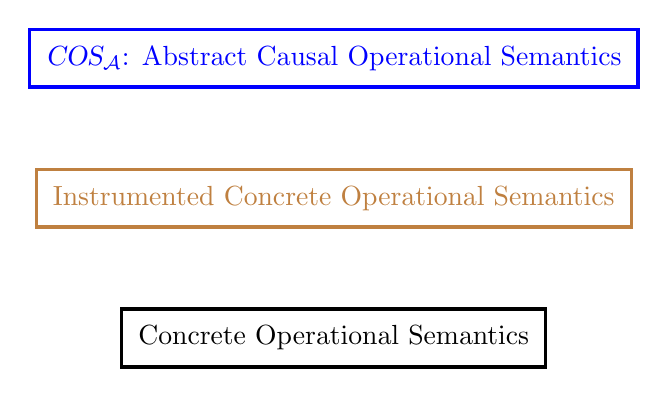
\begin{tikzpicture}[rect/.style = {draw, very thick, rectangle, inner sep = 6pt}, % rectangle
  rrect/.style = {rect, rounded corners}, % rounded rectangle
]
  \node (acos) [blue, rect] {\acos: Abstract Causal Operational Semantics};
  \node (icos) [brown, rect, below = of acos] {Instrumented Concrete Operational Semantics};
  \node (cos) [rect, below = of icos] {Concrete Operational Semantics};
\end{tikzpicture}
\end{document}
